\documentclass{article}
\usepackage[margin=1in]{geometry}
\usepackage{fancyhdr}
\usepackage{graphicx}
\usepackage{vhistory}
\usepackage[parfill]{parskip}
\graphicspath{{../Images/}}

% Set fancy looking header/footer and move page number to the right
\pagestyle{fancy}
\fancyhead{}
\fancyfoot{}
\fancyfoot[R]{\thepage}

\title{}
\author{}
\date{}

\begin{document}
    \pagenumbering{gobble}
    \begin{titlepage}
    \begin{center}
        \vspace*{1cm}

        \Huge
        \textbf{User's Guide for Cloud Backup}

        \vspace{.5cm}
        \LARGE
        Captain CyBeard: Neil Before Us

        \vspace{1cm}

        \textbf{Ryan Breitenfeldt \textbar\ Noah Farris\\ Trevor Surface \textbar\ Kyle Thomas}

        \vspace{.2cm}
        \Large
        May 4, 2020

        \vspace{2cm}
        
\includegraphics[scale=1]{logo}

        \vfill

        Washington State University Tri-Cities\\
        CptS 423 Software Design Project 2

    \end{center}
\end{titlepage}



    \listoffigures

    \newpage
    \pagenumbering{arabic}

    \begin{figure}[h]
    
\includegraphics[scale=.25]{p1}
        \caption{The login page}
    \end{figure}

    \begin{figure}[h]
    
\includegraphics[scale=.25]{p2}
        \caption{User name and password filled out.}
    \end{figure}

    \begin{figure}[h]
    
\includegraphics[scale=.25]{p3}
        \caption{Logged in and ready to enter URL to cloud platform.}
    \end{figure}

    \begin{figure}[h]
    
\includegraphics[scale=.25]{p4}
        \caption{Cloud platform entered.}
    \end{figure}

    \begin{figure}[h]
    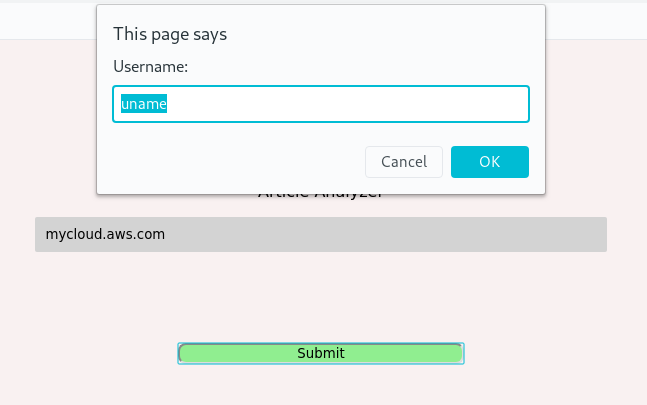
\includegraphics[scale=.55]{p5}
        \caption{Popup prompting for user name.}
    \end{figure}

    \begin{figure}[h]
    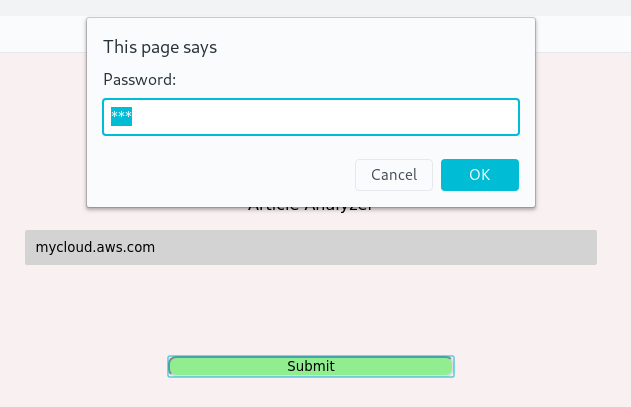
\includegraphics[scale=.55]{p6}
        \caption{Popup prompting for password (note the real application will have the username and password in the same popup or window).}
    \end{figure}

    \begin{figure}[h]
    
\includegraphics[scale=.25]{p7}
        \caption{Displays to user available files to download.}
    \end{figure}
    
    \begin{figure}[h]
    
\includegraphics[scale=.25]{p8}
        \caption{All files selected to be downloaded.}
    \end{figure}

    \begin{figure}[h]
    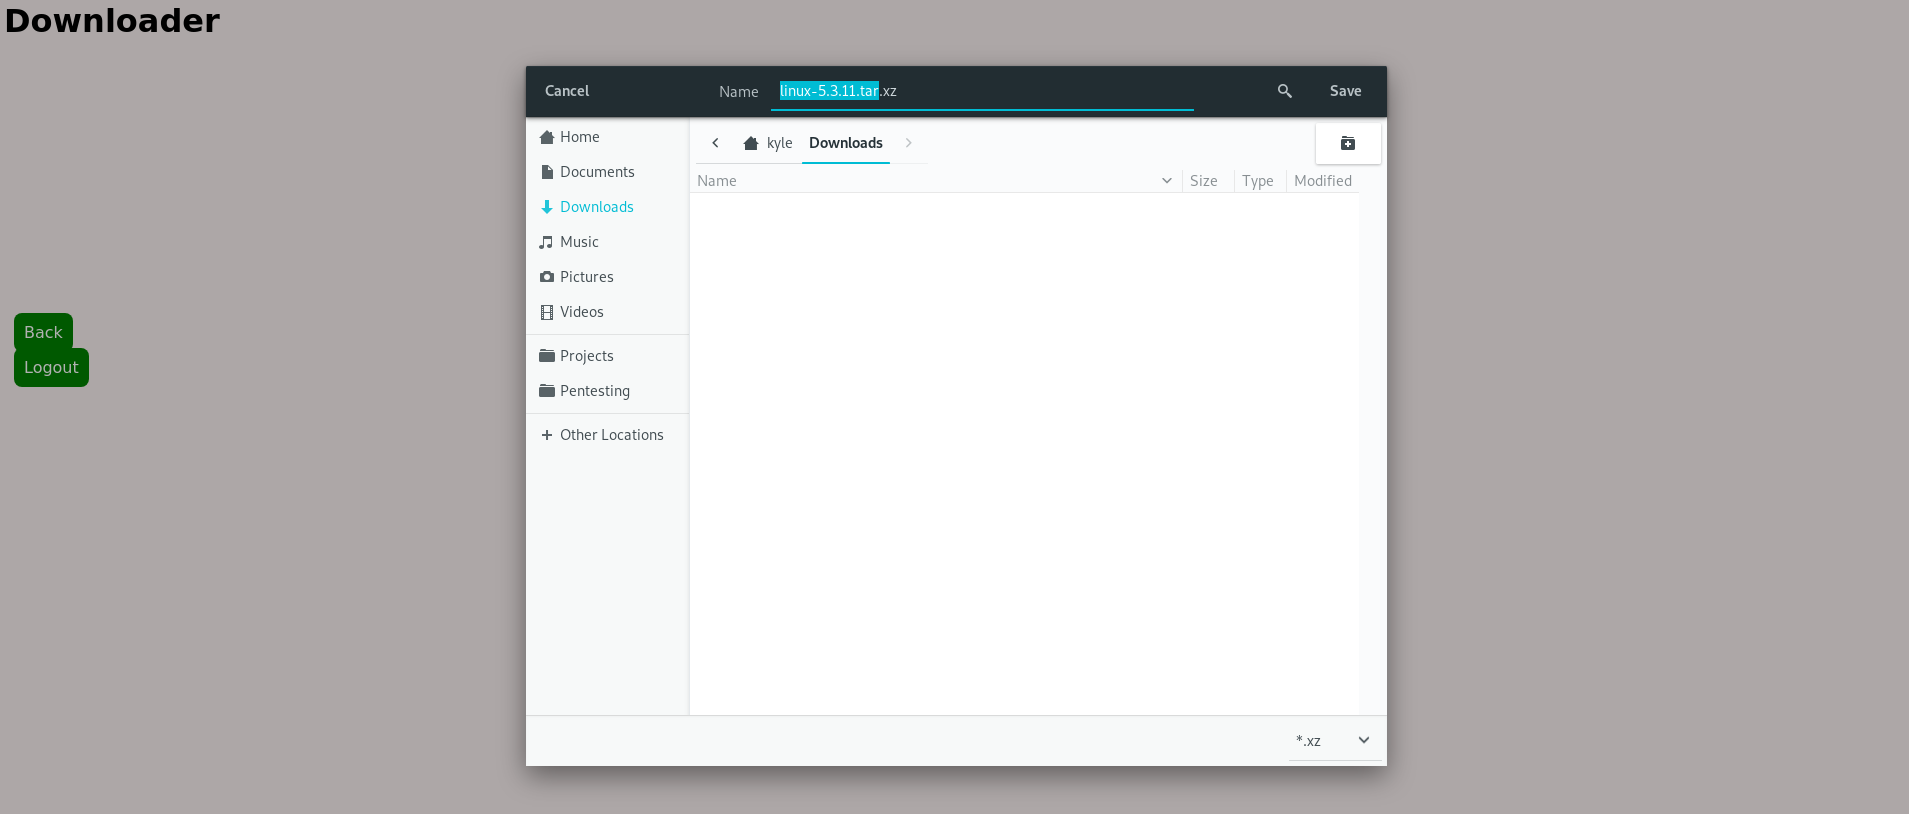
\includegraphics[scale=.25]{p9}
        \caption{Web browser asks where to save downloads.}
    \end{figure}

\end{document}
